\section{Technologies}
In Formula 1, each car is equipped with over 300 sensors, generating 1.1 million datapoints between the racetrack and the pits\cite{DCFrontier}. Through the years, Formula 1 has adopted new technologies and have traditionally been on the forefront of wireless technology. Different proprietary WiFi solutions have been used for telemetry between the cars on the track, and recently, 5G has been adopted to be used for telemetry\cite{FastCompany}. As 5G is still relatively new, we may not have coverage at the track, so it is safer to base this discussion on 4G/LTE.

\subsection{LTE}
LTE has one big advantage over LoRa, in that it has a much higher bitrate at 300 Mbps download and 75 Mbps upload, or even higher with newer LTE technology\cite{MobilePDF}. With such a high bit rate, it should be possible to send and receive much more detailed data. In a car, it would mean that one could have more sensors on the car, or increase the frequency at which values are updated. 4G/LTE is however working on a network, and the system built for the car will be reliant on stable operation of the network, and that the network won't be overpopulated with clients. This will vary from place to place. Typically, solutions with LTE is sending the data to a server on the internet, which is then accesible on a laptop, from which the data can be read and used. A lot of subsystems is needed for this to work, and the setup could be complicated. Furthermore, as LTE exist in one of the commercial frequency spectrums, and server functionality may be subsciption based also, there could be a continuous economic expense.\newline

\subsection{LoRaWAN}
LoRa and LoRaWAN are two different things not to be confused; LoRa is the physical layer level, the transmitting technology, while LoRaWAN is a Data Link layer protocol. LoRaWAN is optimized for low power consumption primarily for battery powered IoT devices. Typically, a pool of end devices are laid out in a star-of-stars topology, connected to a central gateway that links the end devices with a network server. Communication between end devices and gateway is radiocommunication, while communication between gateway and network server would be IP connected\cite{datalink}. LoRa operates in the sub GHz band, with a number of channels spread out over this band. These channels have different bandwidths, and some are uplink while others are downlink. Most of these channels have a 125 KHz bandwidth, while a few have 250- or 500 KHz bandwidth. Within these bands, communication are provided with a special chirp modulation technique proprietary to LoRa\cite{LPWAN}. An end device have a few rules to obey by; The end device should change channel for every transmission, making the system more robust to interference. The end device should change its transmit periodicity, preventing syncronization between end devices. Finally, an end device should comply with local regulations. For example, the open band in EU is different to the one in the US, and there are different rules for transmit duty cycles. Within the LoRaWAN specification there are three different classes of end devices, whereas most are class A. Class A devices have bi-directional communication, where an end devices uplink transmission is followed by a downlink acknowledge message. The end device is ``awake'' in the transmission time and two following windows for receiving confirmation of succesfull transmission. If the message is acknowledged, the end device can go to sleep, wherein the powersaving aspect is. This is an example of an ALOHA type protocol with small time variations in transmission periodicity\cite{datalink}.

\subsection{LoRa and Peer-to-Peer}
While LoRaWAN is network based, LoRa technology can also be used on a peer-to-peer (P2P) basis, that is that two devices can talk directly. This is done by utilizing the LoRa physical layer and the way radio communication is done here. The beforementioned chirp modulation, see figure \ref{fig:chirp}, is a series of chirps where the frequency is sweeped across the channel bandwidth a number of times with varying direction. This way of modulation makes is easier to decode the signal even if it is has lower amplitude, and is actually under the noise floor\cite{LPWAN}\cite{nordal}.\\

LoRa works in a unlicensed band, so a system can be build with no continuous economic expenses. The main limitation of using the 868MHz band is that there are dutycycle regulations, instated by EU. A node can transmit only 1\% of the time. That means, that for the time it takes to transmit a message, the sender should be quiet 99 times that time afterwards. This of course puts a limitation to rate at which messages are send, or it limits the length of messages to reduce transmission time.

\begin{figure}[h!]
  \centering
  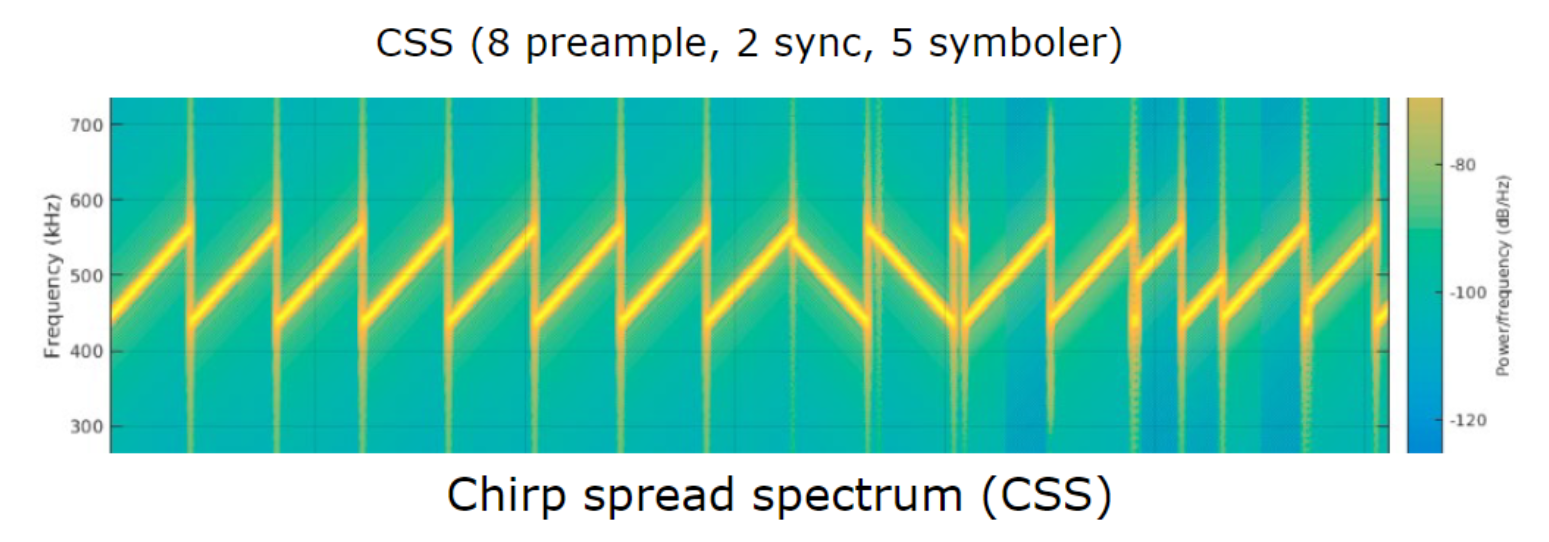
\includegraphics[height = 5cm]{chirp.png}
  \caption{Chirp frequency modulation, proprietary to LoRa}
  \label{fig:chirp}
\end{figure}
